\documentclass[aip,jcp,reprint,floatfix,superscriptaddress]{revtex4-2}
\usepackage{amsmath,amssymb,booktabs,graphicx,color,hyperref}
\graphicspath{{figs/}}
\newcommand{\Tr}{\mathrm{Tr}}
\newcommand{\Mat}{\mathrm{Mat}}
\newcommand{\dd}{\mathrm{d}}
\newcommand{\ad}{a^\dagger}

\begin{document}
\title{A positivity-preserving, thermalizing equation of motion for the two-electron reduced density matrix}

\author{John Parkhill}
\email{john.parkhill@gmail.com}
\affiliation{(affiliation)}

\date{\today}

\begin{abstract}
Truncations of the reduced-density-matrix (BBGKY) hierarchy beyond mean field are unstable: with the three-body cumulant set to zero the two-electron reduced density matrix (2-RDM) leaves the $N$-representable set and diverges within a few femtoseconds. We show that this is not an accident of any particular reconstruction but a structural feature---the truncated flow is the exact dynamics of a non-existent state---and then construct an equation of motion that is stable. Three ingredients are needed. (i) The $\lambda_3=0$ flow is written in closed algebraic form as a sum of a pair-space commutator, a particle--particle ladder sandwich with the Bethe--Goldstone phase-space factor $(1-n_p-n_v)V$, a particle--hole ring term with the $(n_p-n_q)V$ structure, and a contraction term; every piece is polynomial in $(\gamma_1,\gamma_2,V)$, so the flow is Lipschitz and extensive by construction and never forms $\gamma_3$. (ii) Positivity of the $D$, $Q$ and $G$ conditions is enforced by a smooth, dynamical correction in the spirit of Car--Parrinello: an auxiliary Hermitian pair matrix relaxes toward the minimum-norm correction that keeps the flow tangent to the three cones, with a softplus barrier on negative eigenvalues; unlike a projection, this leaves the linear-response spectrum intact. (iii) A bath is derived once at the level of the density operator (Born--Markov, secular in the instantaneous mean-field basis, hence completely positive and quadratic) and contracted consistently to every rank; the rank-2 dissipator is linear in $\gamma_2$ and $\gamma_3$ and is closed with the same $\lambda_3=0$ as the reversible part. On H$_4$ the closed equation propagates for 4.8~fs with all three cones held to $10^{-5}$, 2-RDM errors of 8--12\% without secular growth, and a dipole spectrum whose dominant pole agrees with full configuration interaction to 0.002~Ha; the previous best reconstruction is 0.025~Ha low with spurious lines. With the bath, an uncorrelated determinant thermalizes to a strict fixed point in 2.4~fs, within 2.4\% of the exact dynamics under the same bath model, all cones strictly inside. Every structural ingredient is verified at rank~3 as well, so the construction is order-general. The cost is $O(M^6)$ per time step, independent of the electron number.
\end{abstract}

\maketitle

\section{Introduction}
The one-electron reduced density matrix (1-RDM) equation of motion closed at mean field is stable for a reason that is easy to state and easy to lose sight of: it is the exact dynamics of a family of states (Slater determinants), and the reduced density matrices of a state are automatically $N$-representable. Every attempt to go one rank higher by truncating the cumulant expansion---setting the three-body cumulant $\lambda_3$ to zero and propagating the 2-RDM---has no such family behind it. A state with $\lambda_2\neq 0$ and $\lambda_3=\lambda_4=\cdots=0$ does not exist (the fermionic analogue of Marcinkiewicz's theorem \cite{marcinkiewicz1939,rajagopal1974}), so the truncated flow is not confined to any representable manifold, and in practice it leaves the positive cone and diverges \cite{akbari2012}. Our own earlier attempt (``EE2'', unpublished) failed in exactly this way, and the present work began as an effort to understand why the rank-1 theory of Ref.~\onlinecite{nguyen2015}---a dissipative 1-RDM equation whose Pauli blocking factors keep $0\le\gamma_1\le 1$ invariant and drive the occupations to Fermi--Dirac---does not transfer to rank~2.

The prior art is substantial. Reconstructions of $\gamma_3$ from $\gamma_1$ and $\gamma_2$ go back to Valdemoro, Nakatsuji and Yasuda, and Mazziotti \cite{nakatsuji1996,mazziotti1998,kutzelnigg1999}; time-dependent 2-RDM propagation with purification steps has been developed by Lackner \emph{et al.}\ \cite{lackner2015,lackner2017} and by Bonitz and co-workers in the G1--G2 scheme \cite{joost2020,joost2022}; contraction-consistent reconstructions with the Lackner correction and the recent reconstruction of Ref.~\onlinecite{mueller2405} are the best one-shot closures we know of. All of them stabilize the dynamics by a projection or a purification applied to the state, and none of them, to our knowledge, retains a well-defined linear-response spectrum while doing so. The positivity conditions themselves ($D$, $Q$, $G$; $T_1$, $T_2$) are those of Coleman, Garrod--Percus and Erdahl \cite{coleman1963,garrod1964,mazziotti2007}.

This paper does four things. Section~\ref{sec:structure} analyzes the exact rank-2 flow as a flow on the pair-space matrix $X=\Mat_2$ and shows which part of it moves the spectrum of $X$ and hence threatens positivity. Section~\ref{sec:f0} derives the complete $\lambda_3=0$ flow in a closed channel form. Section~\ref{sec:delta} introduces the smooth dynamical positivity correction and reports 4.8~fs propagations and spectra against full configuration interaction (FCI). Section~\ref{sec:bath} derives the bath and reports thermalization. Section~\ref{sec:rank3} records the rank-3 checks. Every derivation in this paper was carried out with two independent symbolic routes (plain Wick reordering and Mukherjee--Kutzelnigg generalized normal ordering \cite{kutzelnigg1997,mukherjee1997}) validated against exact Fock-space linear algebra to $10^{-15}$; the code and the complete episodic record are in the repository accompanying this paper \cite{repo}.

\section{The rank-2 flow as a flow on pair space}\label{sec:structure}

\subsection{Notation}
$M$ spin-orbitals, $N$ electrons, $\gamma_1[p,q]=\langle\ad_p a_q\rangle$, $\gamma_2[p,v,q,w]=\langle\ad_p\ad_v a_w a_q\rangle$ (ket indices $p,v$; bra indices $q,w$), $\lambda_2=\gamma_2-\gamma_1\wedge\gamma_1$ with $(a\wedge b)[pvqw]=a[pq]b[vw]-a[pw]b[vq]$. $H=\sum h_{pq}\ad_p a_q+\tfrac14\sum V_{pvqw}\ad_p\ad_v a_w a_q$ with antisymmetrized $V$. Pair space is indexed by sorted pairs $(p<v)$, $n_P=M(M-1)/2$; $X[(pv),(qw)]=2\gamma_2[p,v,q,w]$ is Hermitian and positive semidefinite (it is the Gram matrix of the vectors $a_v a_p|\Psi\rangle$). For a one-body matrix $A$, $A\oplus A$ denotes its pair-space lift, $(A\oplus A)[(pv),(qw)]=A_{pq}\delta_{vw}+A_{vw}\delta_{pq}-A_{pw}\delta_{vq}-A_{vq}\delta_{pw}$. $K_h=h\oplus h$, $K_V[(pv),(qw)]=V_{pvqw}$, $N_{\rm op}=\gamma_1\oplus\gamma_1$. $W_{pq}=\sum_{rs}V_{prqs}\gamma_1[r,s]$ is the mean field and $C_{pq}=\sum_{rtu}V_{rtpu}\lambda_2[r,t,q,u]$ the rank-1 collision matrix. The particle--hole (G-matrix) arrangement of a four-index tensor is $\mathrm{ph}(T)[(p,q),(v,w)]=T[p,v,q,w]$, an $M^2\times M^2$ matrix.

\subsection{Drift and collision}
Every Wick term of $\dd\gamma_2/\dd t=i\langle[H,\ad_p\ad_v a_w a_q]\rangle$ contains either $\gamma_2$ or $\gamma_3$, never both, so
\begin{equation}
\frac{\dd X}{\dd t}=D[X]+\Phi[\gamma_3],\qquad D[X]=i[K_h+K_V,\,X].
\label{eq:split}
\end{equation}
That the drift is exactly a commutator with the two-particle cluster Hamiltonian $K_h+K_V$ we verified at $10^{-16}$ on twelve exact states (pure, thermal, quenched). Consequently $D$ conserves the spectrum of $X$, and \emph{all} spectral motion---all positivity risk---resides in the collision part $\Phi$, which is linear in $\gamma_3$. The fraction of the exact flow that is spectral (block-diagonal in the eigenbasis of $X$, hence not representable by any commutator) is 0.1--1.6\% near equilibrium and 13--35\% after an interaction quench: the geminal occupations genuinely move. Mean-field theory is stable not because occupation motion is small but because a commutator cannot move it at all.

The exact flow of any Gram matrix has the form $\dot X=i(S^\dagger X-XS)$ \cite{xr}; in the eigenbasis of $X$, $\dot X_{ij}=iK_{ij}(x_j-x_i)-\tfrac12\Gamma_{ij}(x_i+x_j)$ with $S=K-i\Gamma/2$, so the rate vanishes on the null space of $X$ for any $S$. This is why the exact dynamics is tangent to the positive cone, and it is the property every closure has to reproduce.

\section{The $\lambda_3=0$ flow in closed form}\label{sec:f0}
Substituting the cumulant expansion $\gamma_3=\mathcal A_3(\gamma_1\gamma_1\gamma_1)+\mathcal A_3(\gamma_1\lambda_2)+\lambda_3$ into $\Phi$ and identifying each product class as matrix products in pair or particle--hole space (by common-coefficient fits across pure, thermal and quenched states, then verified directly without fitting at $10^{-15}$ on eight states), we find
\begin{align}
D+\Phi[\gamma_3]_{\lambda_3=0}&=i[K_h+K_V,X]+i(S^\dagger X-XS)+i(Q_C-Q_C^\dagger)+\Phi_{\rm ph},\label{eq:F0}\\
S&=W^{\!\top}\!\oplus W^{\!\top}-K_V N_{\rm op},\qquad
Q_C=\tfrac12\{N_{\rm op},K_C\}-K_{\gamma C}-K_{C\gamma},\nonumber\\
\Phi_{\rm ph}&=2i\big[\mathrm{back}(P_1+P_2-P_3-P_4)-{\rm h.c.}\big],\quad
P_1=\mathrm{Sw}(\gamma_1^{\!\top}\!\otimes I)V_d L_d,\ \ P_4=\mathrm{Sw}(I\otimes\gamma_1)V_dL_d,\nonumber
\end{align}
with $V_d=\mathrm{ph}(V)$, $L_d=\mathrm{ph}(\lambda_2)$, $P_{2,3}$ the right-acting partners, $\mathrm{Sw}$ the within-pair swap, and $\mathrm{back}$ the antisymmetrized return to pair space. We call this flow $F_0$.

Three remarks. First, $K_V N_{\rm op}$ is the Bethe--Goldstone phase-space factor $(1-n_p-n_v)V$ of the particle--particle ladder, and the generator $(\gamma_1^{\!\top}\!\otimes I-I\otimes\gamma_1)V_d$ of $\Phi_{\rm ph}$ is the $(n_p-n_q)V$ structure of the particle--hole ring (RPA/GW) \cite{fetter,ringschuck}; the $\lambda_3=0$ closure is these two channels plus a contraction term, and nothing else. Second, the anti-Hermitian part of $S$, $\Gamma=i[N_{\rm op},K_V]$, is where the mean-field-level flow moves occupations; the two channels are each larger than their sum and cancel strongly, so neither is a closure alone. Third, every term is a polynomial in $(\gamma_1,\gamma_2,V)$: the flow is Lipschitz, size-extensive (connected), costs $O(M^6)$, and never forms the $M^6$ tensor $\gamma_3$.

$F_0$ is the exact dynamics of $\lambda_3=0$ and it reproduces the EE2 failure: from a dipole-kicked ground state of H$_4$ it leaves the $D$, $Q$ and $G$ cones monotonically and diverges at 2.7~fs (Fig.~\ref{fig:spectra}, grey). Positivity restoration by projection at each step \cite{lackner2015,joost2022} stabilizes it but, as we verified explicitly, destroys the linear-response spectrum: the projected flow is not a smooth function of the state.

\section{A smooth dynamical positivity correction}\label{sec:delta}
Let $P\in\{D,Q,G\}$ denote the three Gram cones,
$D=X/2$, $Q[(pv),(qw)]=\langle a_pa_va^\dagger_wa^\dagger_q\rangle$, $G[(pq),(rs)]=\langle\ad_pa_q\ad_sa_r\rangle=\delta_{qs}\gamma_1[p,r]-\gamma_2[p,s,r,q]$, all affine in $(\gamma_1,\gamma_2)$ (verified against direct Gram matrices at $10^{-16}$), so that any pair-space flow $F$ induces linear rates $\dot P(F)$. We augment the state by a Hermitian pair matrix $\delta$ and propagate
\begin{align}
\frac{\dd X}{\dd t}&=F_0(X)+\delta,\label{eq:dyn1}\\
\tau\frac{\dd\delta}{\dd t}&=-(\delta-\delta_{\rm hard})-\Pi_\perp\!\Big[\kappa_{\rm neg}\sum_P\sum_i b'(x_i^P)\,\dot P^\dagger(u_i^Pu_i^{P\dagger})\Big],\label{eq:dyn2}
\end{align}
where $(x_i^P,u_i^P)$ are the eigenpairs of cone $P$, $b(x)=\epsilon^2\,\mathrm{softplus}(-x/\epsilon)^2$ is a $C^\infty$ barrier that vanishes exponentially inside the cone and grows as $x^2$ outside, $\dot P^\dagger$ is the adjoint of the cone-rate map, $\delta_{\rm hard}$ is the minimum-norm correction enforcing that $\Tr_2(F_0+\delta)/(N-1)$ equals the exact rank-1 equation of motion (which contains no $\gamma_3$) and that the energy is conserved, and $\Pi_\perp$ projects the barrier force onto the complement of those constraints. Equation~\eqref{eq:dyn2} is a Car--Parrinello-like relaxation \cite{car1985}: as $\tau\to0$ it reduces to the projection; for finite $\tau$ the closure is a smooth ODE, so it has a linear-response spectrum, and the fictitious modes sit at $\mathrm{Re}\,\omega\approx-1/\tau$ well outside the physical window. We first used a spectral-function tangency potential in addition to the barrier; a $2\times2$ test showed the barrier alone gives the identical trajectory to three digits, so Eq.~\eqref{eq:dyn2} is the final form. All forces are obtained through adjoint maps, never by rotating a basis of $O(M^4)$ perturbations, which brings the cost from $O(M^{10})$ in our first implementation to $O(M^6)$ time and $O(M^4)$ memory per evaluation, independent of $N$; on an RTX~3090 one right-hand side takes 20--35~ms from $M=8$ to $M=14$.

\subsection{Results: 4.8 fs on H$_4$}
System: H$_4$ in an asymmetric trapezoid (sides 0.80 and 1.20~\AA), STO-3G, $M=8$, $N=4$; initial state $e^{-i0.3\mu_x}|\Psi_0\rangle$ with $|\Psi_0\rangle$ the FCI ground state, kicked at the wavefunction level; RK4 with $\Delta t=0.005$~a.u.\ ($\Delta t$-halving checked); 200~a.u.~$=4.84$~fs; compared with exact FCI propagation at every 0.5~a.u. Parameters $\tau=0.5$~a.u., $\kappa_{\rm neg}=10^4$, $\epsilon=10^{-3}$.

\begin{table*}[t]
\caption{4.84~fs propagations of x-kicked H$_4$. Minimum eigenvalue of $D$ over the run, relative Frobenius error of $\gamma_2$ against exact FCI at 100 and 200~a.u., energy drift.}
\begin{ruledtabular}\begin{tabular}{lcccl}
closure & min eig $D$ & $e(\gamma_2)$ 100/200 a.u. & $|\Delta E|$ & fate\\\hline
$F_0$ ($\lambda_3=0$) & $-0.5$ at 100 a.u. & 0.24 / --- & $5\times10^{-3}$ & diverged at 2.7 fs\\
Ref.~\onlinecite{mueller2405} $+$ Lackner & $-0.05$ & 0.27 / 0.17 & $10^{-14}$ & stable, inaccurate\\
Eqs.~(\ref{eq:dyn1},\ref{eq:dyn2}), $\kappa_{\rm neg}=10^4$ & $+1.7\times10^{-3}$ & 0.11 / 0.16 & $5\times10^{-6}$ & stable\\
Eqs.~(\ref{eq:dyn1},\ref{eq:dyn2}), $\kappa_{\rm neg}=10^5$ & $+5\times10^{-4}$ & 0.12 / 0.13 & $10^{-5}$ & stable\\
\end{tabular}\end{ruledtabular}
\label{tab:traj}
\end{table*}

\begin{figure*}[t]
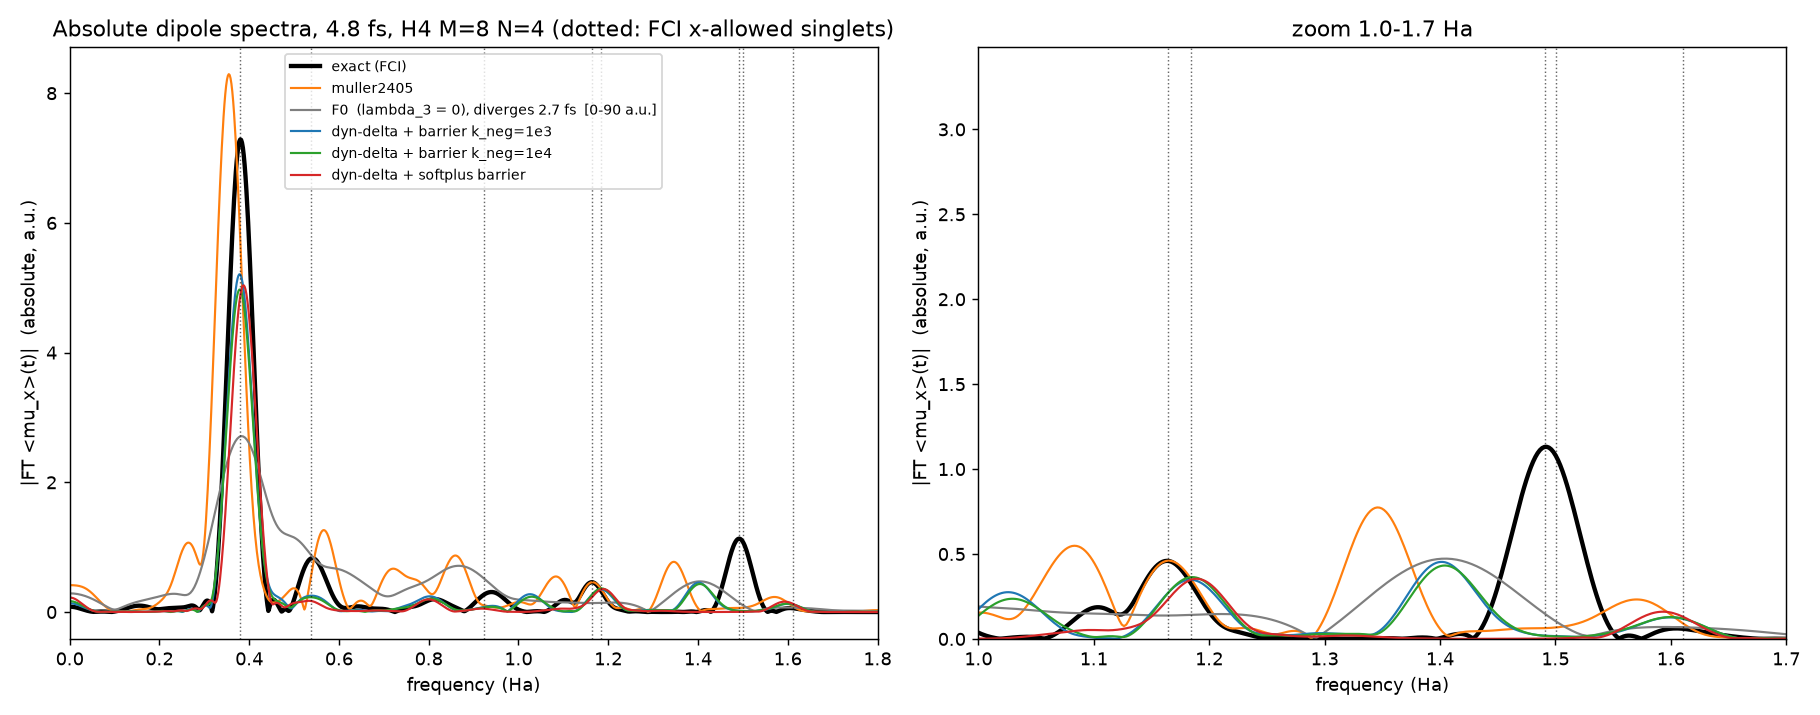
\includegraphics[width=\textwidth]{dipole_spectra_absolute.png}
\caption{Absolute dipole spectra, $|\mathcal F[\langle\mu_x\rangle(t)-\bar\mu]|$ with a Hann window over 4.84~fs, x-kicked H$_4$ ground state. Black: exact FCI. Dotted: FCI x-dipole-allowed singlet excitations. The closures of Eqs.~(\ref{eq:dyn1},\ref{eq:dyn2}) (blue, green, red) place the dominant pole at 0.378~Ha (exact 0.380) with the correct width and no spurious structure below 1.3~Ha; the Ref.~\onlinecite{mueller2405} reconstruction (orange) is 0.025~Ha low, broadened, and carries four spurious lines; $F_0$ (grey, before divergence) is broadened everywhere. All approximate closures place the 1.49~Ha pole about 0.1~Ha low. Right: zoom of the 1.0--1.7~Ha region.}
\label{fig:spectra}
\end{figure*}

The closure holds all three cones for the full 4.8~fs, conserves the trace exactly and the energy to $10^{-5}$, and its 2-RDM error oscillates between 8 and 12\% without secular growth; it is about twice as accurate as the best previous reconstruction at every time while $10^3$--$10^4$ times closer to the cone. In the dipole spectrum (Fig.~\ref{fig:spectra}) the dominant pole is reproduced to 0.002~Ha with the correct width. The linear-response spectrum, computed independently by linearizing the extended $(X,\delta)$ system at the FCI ground state and matching modes to FCI transition densities by biorthogonal projection, gives a mean error of 0.055~Ha over the six lowest singlets (0.059 for $F_0$; 0.94 for the projected version, which has no spectrum). In a mixed-state (thermal, $kT=0.5$) linear-response row the channel form $F_0$ gives 0.044~Ha against 0.074 for Ref.~\onlinecite{mueller2405}---the ranking reverses away from pure ground states, which the one-shot reconstruction was tuned to.

\section{Dissipation: derived once, contracted to every rank}\label{sec:bath}
The rank-1 theory of Ref.~\onlinecite{nguyen2015} derives a second-order (TCL2) master equation for the density operator $\rho$ with a one-body system--bath coupling $H_{SB}=\sum_\alpha A_\alpha\otimes B_\alpha$, $A_\alpha=\sum_{pq}g^\alpha_{pq}\ad_pa_q$, and contracts it to $\gamma_1$. The same generator contracts to every rank, and doing so consistently is the step that EE2 omitted. With the coupling operator's Heisenberg evolution closed by the instantaneous mean-field one-body Hamiltonian $f=h+W[\gamma_1]$ (approximation A3, the choice made in Ref.~\onlinecite{nguyen2015}) and a secular approximation in the eigenbasis of $f$, the generator is of Davies form \cite{davies1974,breuer2002},
\begin{equation}
\mathcal D[\rho]=\sum_\omega\gamma(\omega)\big(L_\omega\rho L_\omega^\dagger-\tfrac12\{L_\omega^\dagger L_\omega,\rho\}\big),\qquad
L_\omega=\sum_{\epsilon_b-\epsilon_a=\omega}A_{ab}\,\ad_a a_b,
\end{equation}
with one-body jump operators, rates $\gamma(\omega)=2\pi J(|\omega|)[n_B(|\omega|)+\theta(\omega)]$ obeying detailed balance, and an Ohmic $J(\omega)=\eta\omega e^{-\omega/\omega_c}$. It is completely positive at every instant and \emph{quadratic}, so its contraction to rank $k$ is linear in $\gamma_k$ and $\gamma_{k+1}$ and nothing higher---the dissipative hierarchy has the same structure as the reversible one. We verified this directly: with the coupling evolved under $f$, the rank-1 dissipator's response to perturbations that change only $\gamma_3$ is $4\times10^{-12}$; with the coupling evolved under the exact $H_S$ it is 30\%, and for a secular approximation in the many-body energy basis it is 95\%---complete positivity by secularization on $\rho$ cannot be contracted to a closed low-rank equation.

The Wick contraction to ranks 1 and 2 (the rank-$(k+2)$ bare moments cancel identically among the three words $L^\dagger OL-\tfrac12L^\dagger LO-\tfrac12OL^\dagger L$) reproduces the Fock-space generator at $2\times10^{-16}$ and $4\times10^{-16}$; at $V=0$, $\lambda_2=0$ the rank-1 populations reproduce the Pauli master equation of Ref.~\onlinecite{nguyen2015} at $3\times10^{-16}$ (its coherence decay used a further mean-rate simplification). The rank-2 dissipator depends on $\gamma_3$ at $O(1)$---0.38 against a rate norm of 0.33 at a correlated thermal state---and we close it with the same $\lambda_3=0$ as $F_0$, giving $D_2$: 4.1\% from the exact dissipator, trace-preserving to $10^{-15}$, contraction-consistent to 3\%.

\begin{figure*}[t]
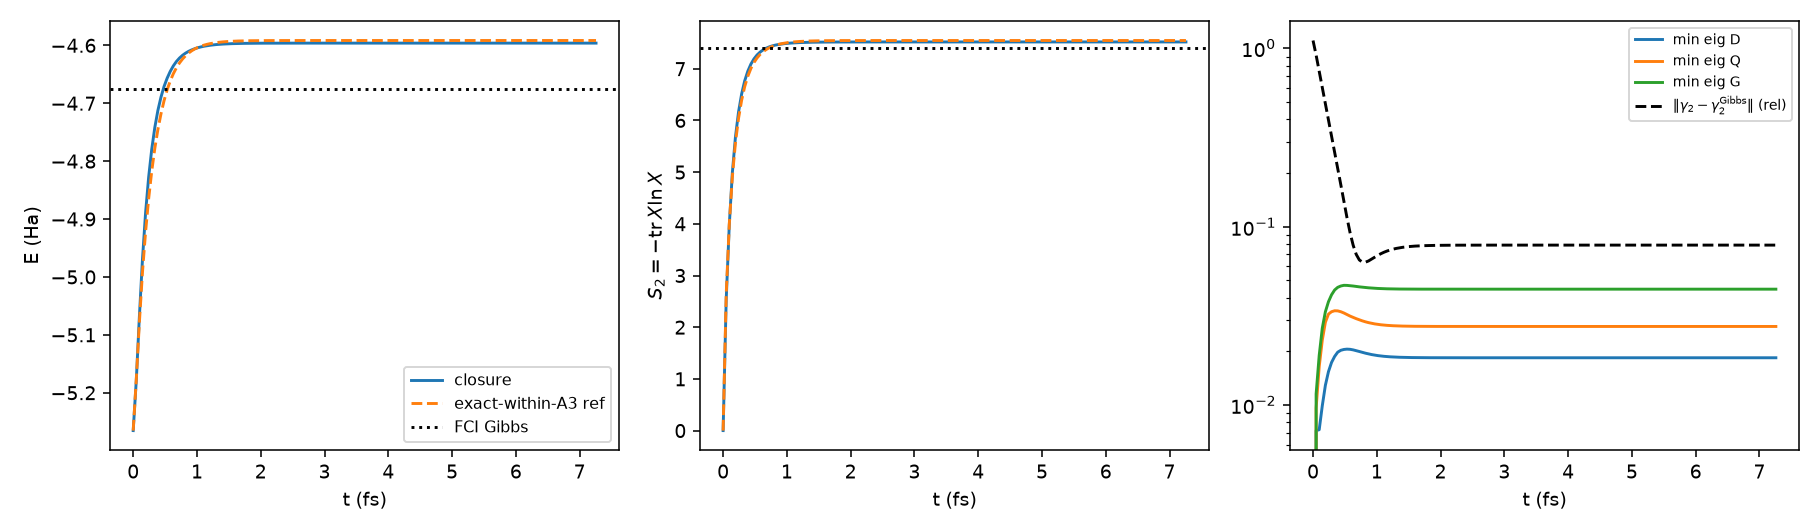
\includegraphics[width=\textwidth]{thermalize.png}
\caption{Thermalization of H$_4$ ($M=8$, $N=4$) from the Hartree--Fock determinant under $F_0+\delta+D_2$ at $kT=0.5$ (Ohmic bath, $\eta=0.05$, $\omega_c=1$, four one-body coupling operators), RK4 $\Delta t=0.01$~a.u., 300~a.u.~$=7.3$~fs. Left: energy; center: pair-space entropy $S_2=-\Tr X\ln X$; right: minimum eigenvalues of $D$, $Q$, $G$ and the distance to the FCI Gibbs 2-RDM. Dashed: the exact propagation of $\rho$ under the same bath model.}
\label{fig:thermal}
\end{figure*}

Figure~\ref{fig:thermal} shows the result. The closed rank-2 equation thermalizes: entropy rises monotonically, a strict fixed point is reached by 100~a.u.\ (2.4~fs) and held for the remaining 5~fs, and all three cones stay strictly inside throughout ($|\delta|=0.004$ at the fixed point; the dissipator itself keeps the state representable). The fixed point is 2.4\% from that of the exact $\rho$-level dynamics under the same bath model, and 7.9\% from the FCI Gibbs state; the exact dynamics under the same bath lands at 8.2\%. The residual is therefore the bath model (A3 evolves the coupling under $f$, so the bath sees a mean-field spectrum and drives toward a state that is too hot by 85~mHa), not the closure, and is removable by evolving the coupling under the effective pair Hamiltonian of Eq.~\eqref{eq:F0} at the cost of $\lambda_4$-closed terms.

Kicking the thermal fixed point with the bath on, the closure's dipole response overlies the exact reference for the full 19~fs propagated (both damped within 0.5~fs at $\eta=0.05$; a weak-bath run resolving the thermal spectrum is in progress and will be reported with the final version).

\section{Order generality: rank 3}\label{sec:rank3}
The programme's requirement is that every structural claim be verified at two adjacent ranks. For rank 3 we find, with no new algebra beyond term-list generation: the drift $\dd\Mat_3/\dd t|_{\gamma_4\to0}$ is exactly $i[K_3,\Mat_3]$ with $K_3$ the explicit three-particle cluster Hamiltonian ($2\times10^{-15}$ on H$_3$ and H$_4$); the rank-3 equation is exact at $N=3$ ($4\times10^{-16}$); the one-body Davies dissipator contracts to rank 3 with $\gamma_3$ and $\gamma_4$ only (27 and 12 terms; $\gamma_5$ moments cancel; $10^{-16}$ against the Fock space); and the five rank-3 Gram cones ($D_3$, $Q_3$, and the mixed $T_1$, $T_2$ of Erdahl) have affine forms in $\gamma_1..\gamma_3$ verified against direct Gram matrices at $6\times10^{-16}$. On H$_4$ the rank-3 collision part $\Phi_3[\gamma_4]$ has norm 1.2 against a drift of 2.05, so $\lambda_4=0$ would be the sole approximation of a rank-3 closure. Assembling and propagating that closure ($O(M^9)$ time, $O(M^6)$ memory) is the immediate next step.

\section{Conclusions}
The instability of cumulant-truncated 2-RDM dynamics is structural: the truncation is not a state. Three moves make it stable without a projection. Writing the $\lambda_3=0$ flow in channel form makes it cheap, Lipschitz and extensive and localizes the positivity risk in the interplay of the ladder and ring channels; a smooth dynamical correction in the Car--Parrinello spirit holds the $D$, $Q$ and $G$ cones while retaining a linear-response spectrum; and a dissipator derived once on $\rho$ and contracted consistently makes the equation thermalize to a representable fixed point. The resulting equation of motion is $O(M^6)$ per step, independent of the number of electrons, and its accuracy limit is now attributable: about half of the three-cumulant's effect on the 2-RDM is fixed by positivity and conservation, the other half is genuine three-body correlation, and the thermal fixed point's error is the bath model rather than the closure. Both are addressed at the next rank, whose structural ingredients are already verified.

What we have not shown: any system beyond H$_3$/H$_4$; propagation beyond 50~fs; exact extensivity of $\delta$ (1--2\% cross-fragment leak from its minimum-norm structure); and a Hamiltonian structure for the corrected flow (its physical poles have $|\mathrm{Re}\,\omega|\le10^{-2}$ empirically, not by construction). The relation of the Gram-matrix factorization of the exact flow to the contracted Schr\"odinger equation and to prior positivity-preserving propagation schemes \cite{mazziotti2006,lackner2015,joost2022} should be examined before any claim of priority is made for it.

\begin{acknowledgments}
(to be written)
\end{acknowledgments}

\begin{thebibliography}{99}
\bibitem{nguyen2015} T.~S. Nguyen, R. Nanguneri, and J. Parkhill, J. Chem. Phys. \textbf{142}, 134113 (2015).
\bibitem{marcinkiewicz1939} J. Marcinkiewicz, Math. Z. \textbf{44}, 612 (1939).
\bibitem{rajagopal1974} A.~K. Rajagopal and E.~C.~G. Sudarshan, Phys. Rev. A \textbf{10}, 1852 (1974).
\bibitem{akbari2012} A. Akbari, M.~J. Hashemi, A. Rubio, R.~M. Nieminen, and R. van Leeuwen, Phys. Rev. B \textbf{85}, 235121 (2012).
\bibitem{nakatsuji1996} H. Nakatsuji and K. Yasuda, Phys. Rev. Lett. \textbf{76}, 1039 (1996).
\bibitem{mazziotti1998} D.~A. Mazziotti, Phys. Rev. A \textbf{57}, 4219 (1998).
\bibitem{kutzelnigg1999} W. Kutzelnigg and D. Mukherjee, J. Chem. Phys. \textbf{110}, 2800 (1999).
\bibitem{lackner2015} F. Lackner, I. B\v{r}ezinov\'a, T. Sato, K.~L. Ishikawa, and J. Burgd\"orfer, Phys. Rev. A \textbf{91}, 023412 (2015).
\bibitem{lackner2017} F. Lackner, I. B\v{r}ezinov\'a, T. Sato, K.~L. Ishikawa, and J. Burgd\"orfer, Phys. Rev. A \textbf{95}, 033414 (2017).
\bibitem{joost2020} J.-P. Joost, N. Schl\"unzen, and M. Bonitz, Phys. Rev. B \textbf{101}, 245101 (2020).
\bibitem{joost2022} J.-P. Joost, N. Schl\"unzen, H. Ohldag, M. Bonitz, F. Lackner, and I. B\v{r}ezinov\'a, Phys. Rev. B \textbf{105}, 165155 (2022).
\bibitem{mueller2405} (author list), arXiv:2405.05093 (2024).
\bibitem{coleman1963} A.~J. Coleman, Rev. Mod. Phys. \textbf{35}, 668 (1963).
\bibitem{garrod1964} C. Garrod and J.~K. Percus, J. Math. Phys. \textbf{5}, 1756 (1964).
\bibitem{mazziotti2007} D.~A. Mazziotti (ed.), \emph{Reduced-Density-Matrix Mechanics}, Adv. Chem. Phys. \textbf{134} (Wiley, 2007).
\bibitem{kutzelnigg1997} W. Kutzelnigg and D. Mukherjee, J. Chem. Phys. \textbf{107}, 432 (1997).
\bibitem{mukherjee1997} D. Mukherjee, Chem. Phys. Lett. \textbf{274}, 561 (1997).
\bibitem{repo} J. Parkhill \emph{et al.}, \texttt{github.com/jparkhill/2rdm\_noneq\_rdm}; see \texttt{docs/COMMUTATOR-STRUCTURE.md} (episodic record), \texttt{docs/DYNDELTA-SPEC.md} (the correction, every ingredient and its cost), \texttt{docs/BATH-DERIVATION.md} (the dissipator), \texttt{docs/PRIOR-ART-TODO.md} (attribution obligations).
\bibitem{xr} \texttt{docs/XR-POSITIVITY.md} in Ref.~\onlinecite{repo}; the relation to Refs.~\onlinecite{mazziotti2006,lackner2015,joost2022} is to be established.
\bibitem{fetter} A.~L. Fetter and J.~D. Walecka, \emph{Quantum Theory of Many-Particle Systems} (McGraw-Hill, 1971).
\bibitem{ringschuck} P. Ring and P. Schuck, \emph{The Nuclear Many-Body Problem} (Springer, 1980).
\bibitem{car1985} R. Car and M. Parrinello, Phys. Rev. Lett. \textbf{55}, 2471 (1985).
\bibitem{davies1974} E.~B. Davies, Commun. Math. Phys. \textbf{39}, 91 (1974).
\bibitem{breuer2002} H.-P. Breuer and F. Petruccione, \emph{The Theory of Open Quantum Systems} (Oxford, 2002).
\bibitem{mazziotti2006} D.~A. Mazziotti, Phys. Rev. Lett. \textbf{97}, 143002 (2006).
\end{thebibliography}

\end{document}
